\newtheorem{theo}{Theorem}

\section{The \ac{ams} algorithm}
\label{app:ams}

This appendix describes the \ac{ams} algorithm, gives a brief summary of the main
mathematical results and discusses its use in practice.
\subsection{Description of the algorithm}
We consider an ensemble of $N$ independent trajectories $\{x_n^{(0)}(t)\}_{1\leq n \leq N}$, for a fixed duration $T_a$.
These trajectories could be generated by any continuous time Markov model: a stochastic process, for instance a diffusion, or a chaotic deterministic dynamical system.

Starting from this initial ensemble, the \ac{ams} consists in a series of iterations in which one or more trajectories are discarded, and re-simulated from a given point in time $t \in [0, T_a]$ to the final time $t = T_a$.

To start off with, each of these trajectories is associated a weight $w_0=1$.
Then, at iteration $j\geq 1$, we evaluate the score of all trajectories $\{x_n^{(j-1)}(t)\}_{1 \leq n \leq N}$ at iteration $j-1$, measured by the maximum of the score function $\xi$ over the whole trajectory:
\begin{equation}
  \mathcal{Q}_n^{(j)} = \sup_{0 \leq t \leq T_a} \xi(t,x_n^{(j-1)}(t)).
\end{equation}
Then, the trajectories corresponding to the lowest $\mathcal{Q}_n^{(j)}$ are selected: we denote $\mathcal{Q}_j^\star= \min_{1\leq n \leq N} \mathcal{Q}_n^{(j)}$ and $n_{j,1}^\star,\ldots,n_{j,\ell_j}^\star$ the indices of trajectories such that:
\begin{equation}
  \label{eq:ams_threshold_def}
  \mathcal{Q}_{n_{j,1}^\star}^{(j)} = \cdots = \mathcal{Q}_{n_{j,\ell_j}^\star}^{(j)} = \mathcal{Q}_j^\star.
\end{equation}
One might expect intuitively that $\ell_j=1$.
However, because of the discretization of the dynamical equations in the numerical model, two or more trajectories may yield the same level $\mathcal{Q}_n^{(j)}$, see~\cite{brehier:hal-01142704}.
The next step is known as the \textit{mutation step}: for each trajectory $x_{n_{j,\ell}^\star}^{(j-1)}$ ($1 \leq \ell \leq \ell_j$), we choose a trajectory $x_{n_\ell}^{(j-1)}$ ($n_{\ell} \neq n_{j,1},\ldots n_{j,\ell_j}$) randomly among the $N-\ell_j$ remaining trajectories, and define the time $t_{j,\ell}$ defined as the smallest time $t$ such that $\xi(t,x_{n_\ell}^{(j-1)}(t))>\mathcal{Q}_j^\star$.
Finally, we define the new replica $x_{n_{j,\ell}^\star}^{(j)}$ by copying the trajectory $x_{n_\ell}^{(j-1)}$ from $t_0$ to $t_{j,\ell}$, and simulating the rest of the trajectory, from $t_{j,\ell}$ to $T_a$.
For a Markov process, for instance a diffusion, a new realisation of the noise is used in order to simulate the new trajectory from $t_j$ to $T_a$.
For a chaotic deterministic system, a small amplitude noise is added to the initial condition at time $t_j$.
The other trajectories are not modified: $x_n^{(j)}=x_n^{(j-1)}$ for $n \neq n_{j,1}^\star,\ldots,n_{j,\ell}^\star$.
The selection-mutation process is illustrated on Fig.~\ref{fig:AMS_schema}.

\begin{figure}
  \centering
  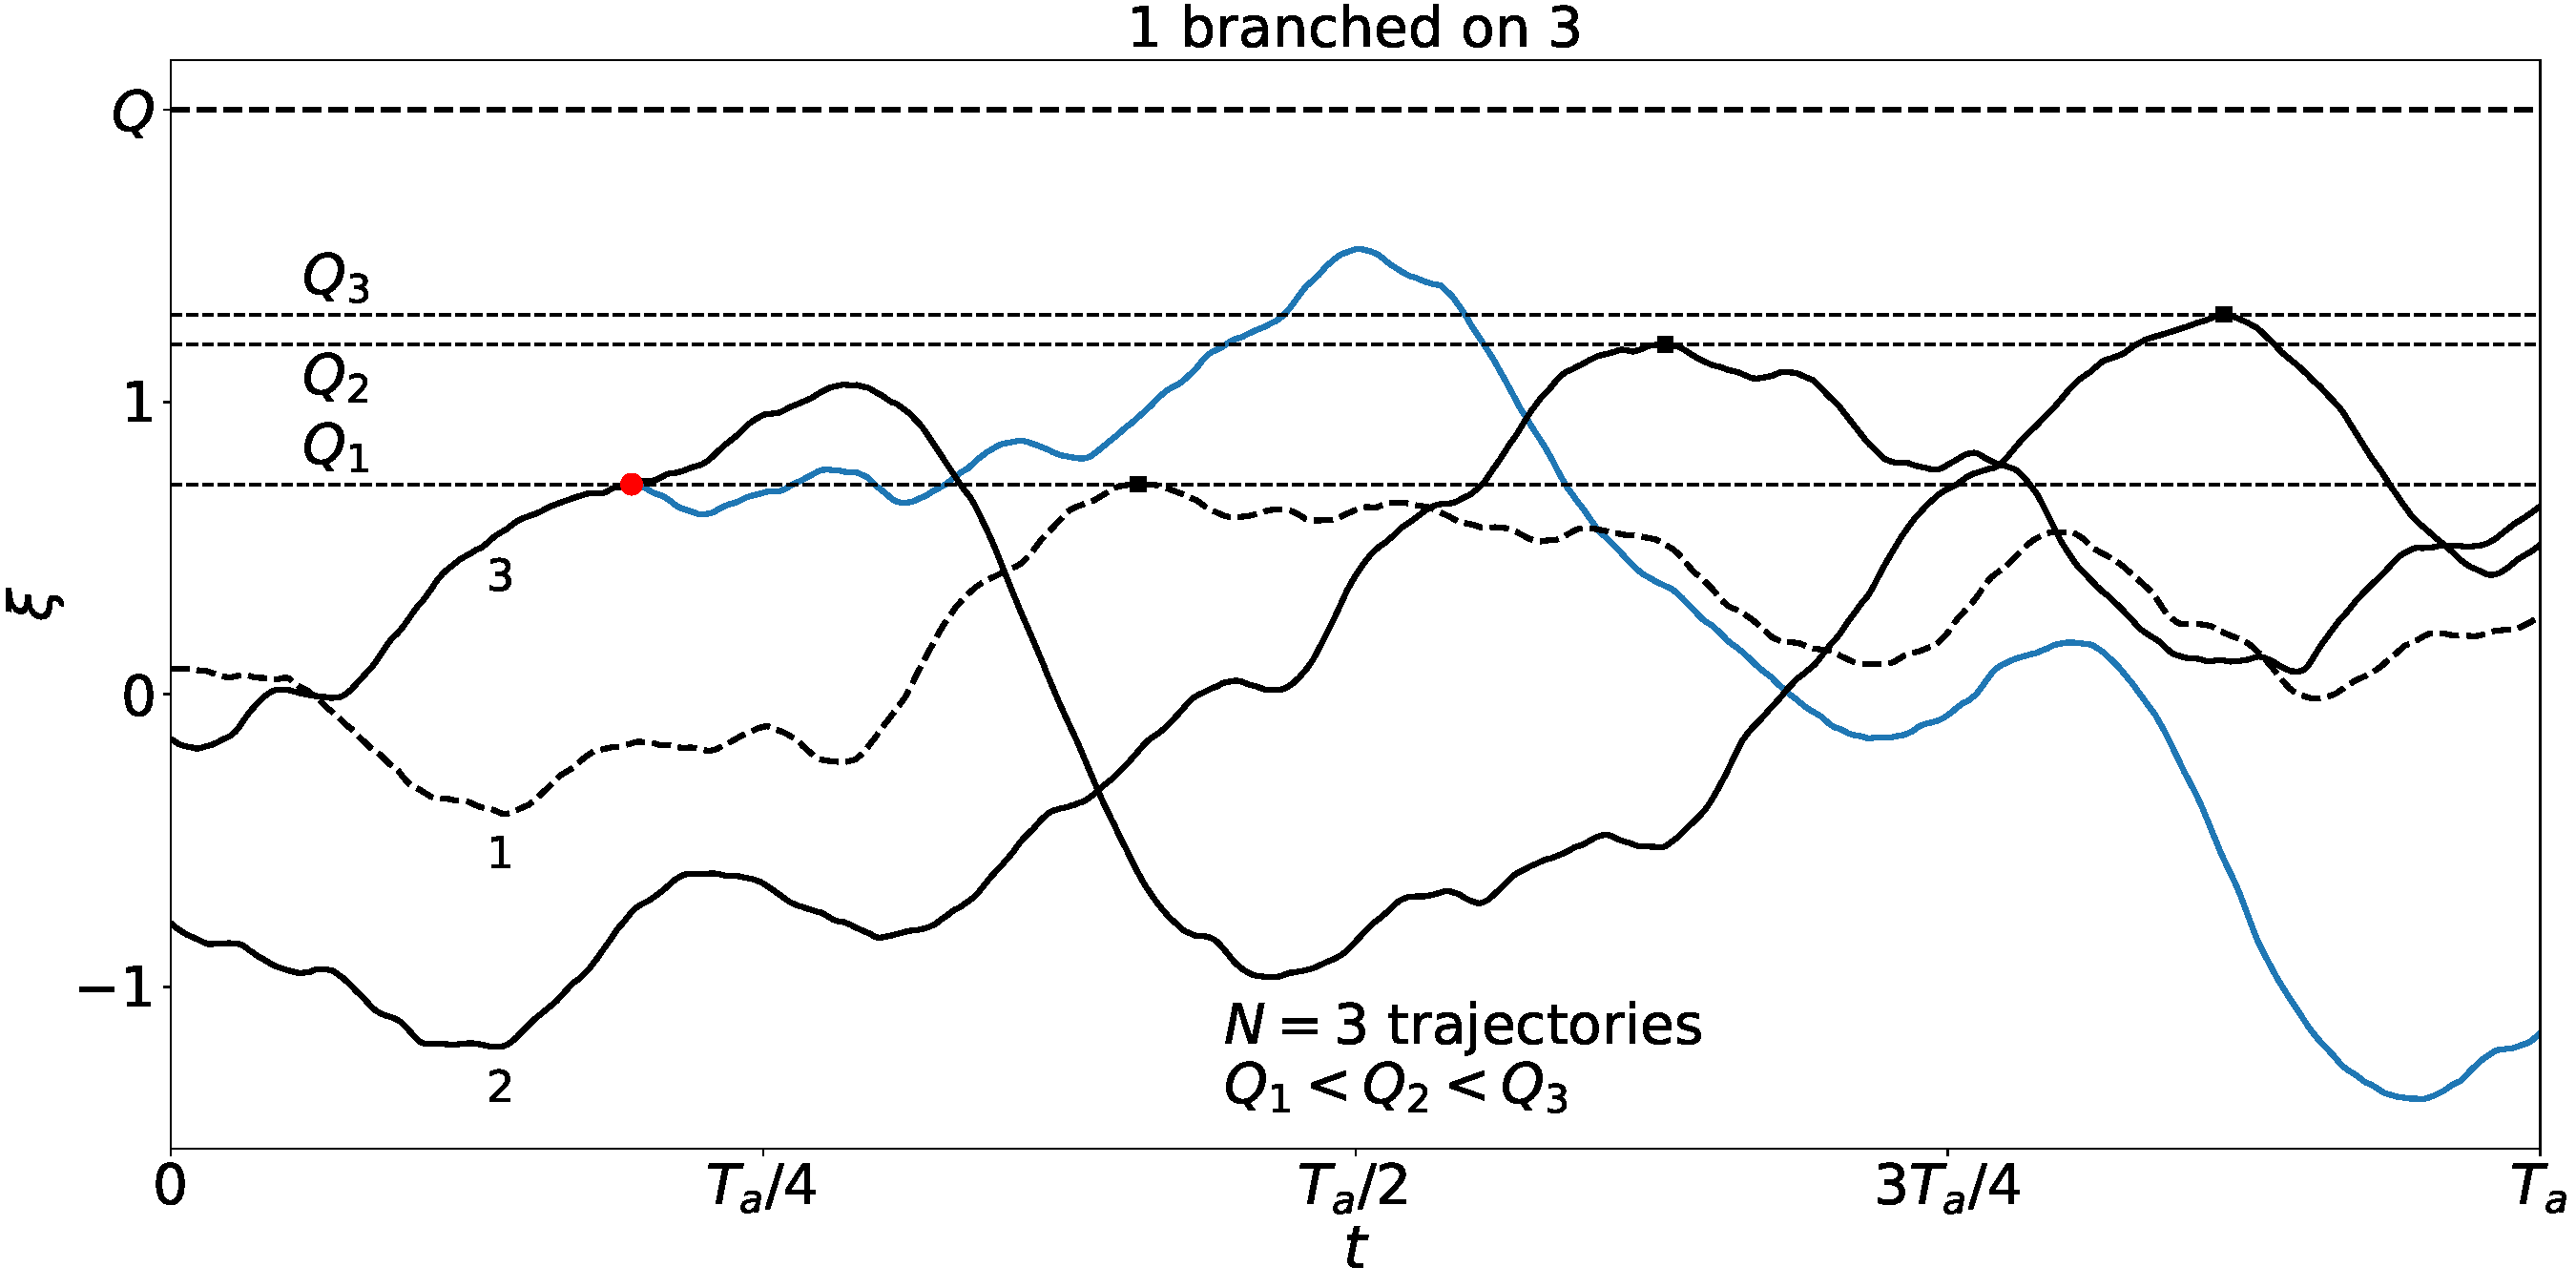
\includegraphics[width=.7\linewidth]{illustr_AMS/illustr_AMS}
  \caption{Illustration of one iteration the \ac{ams} algorithm. Starting from an initial ensemble of 3 trajectories, trajectory 1 is selected as it corresponds to the lowest maximum of the score function $Q_1 = \mathcal{Q}_{j}^\star$. Out of the 2 other trajectories, trajectory 3 is chosen randomly (with probability 1/2) to serve as the base of the resampling of trajectory 1. Trajectory 1 is first made a copy of trajectory 3 from $t=0$ to $t_j$, then simulated from $t_j$ to $T_a$.}
  \label{fig:AMS_schema}
\end{figure}

After $N$ iterations of this selection-mutation procedure, the number of resampled trajectories is
$\tilde{J} = \sum_{j=1}^J \ell_j$.
Ultimately, the algorithm generates $M=N+\tilde{J}$ trajectories, given explicitly by the set $\{x_n^{(0)}\}_{1 \leq n \leq N} \cup \{ x_{n_{j,\ell}^\star}^{(j)}\}_{1 \leq \ell \leq \ell_j, 1 \leq j \leq J}$, or equivalently, the set $\{x_n^{(J)}\}_{1 \leq n \leq N} \cup \{ x_{n_{j,\ell}^\star}^{(j-1)}\}_{1 \leq \ell \leq \ell_j, 1 \leq j \leq J}$.
\subsection{How to compute the probability}
Trajectories $x_n^{(j)}$ forming the ensemble at step $j$ are attributed a weight $w_j$ given by~\cite{Cerou2007,Cerou2011,brehier:hal-01142704}:
\begin{equation}
  w_j = \prod_{i=1}^j \left( 1 - \frac{\ell_i}{N}\right)=\left( 1 - \frac{\ell_j}{N}\right)w_{j-1}.
\end{equation}
This means that each trajectory in the sampled ensemble has an associated weight, given by the iteration until which it was a member of the ensemble: $w_J$ for the final trajectories $\{x_n^{(J)}\}_{1 \leq n \leq N}$, and $w_{j-1}$ for the trajectories $\{ x_{n_{j,\ell}^\star}^{(j-1)}\}_{1 \leq \ell \leq \ell_j, 1 \leq j \leq J}$ resampled at iteration $1 \leq j \leq J$.
Alternatively, $w_0 = 1$ for the initial trajectories, and $w_j$ for the trajectories $\{ x_{n_{j,\ell}^\star}^{(j)}\}_{1 \leq \ell \leq \ell_j, 1 \leq j \leq J}$ resampled at iteration $1 \leq j \leq J$.
Let us relabel these trajectories and their associated weights as $\{(x_m,w_m)\}_{1 \leq m \leq M}$.
Normalising the weights with $W=\sum_{m=1}^M w_m$, we obtain the probabilities $p_m=w_m/W$ associated with the trajectories.
\subsection{Summary of mathematical results}
We now consider the final ensemble of trajectories sampled by the \ac{ams} algorithm, after a given number
of iterations $N$.
We call $a$ the lowest maximum among the trajectories in the ensemble, \textit{i.e.} the final value of the threshold $\mathcal{Q}^{\star}$ defined in Eq.~\eqref{eq:ams_threshold_def}.
The \ac{ams} provides an estimator of the probability that a the maximum of the score function over a trajectory of duration $T_a$ is above $a$, that is:
\begin{equation}
  \label{eq:estimator_ams}
  q(a) = \mathbb{P}\left[ \underset{0\leq t \leq T_a}{\max} \xi(\mathbf{x}, t) > a \right]
\end{equation}
In the following we denote this estimator $\hat{q}_N(a)$.
One of the main properties of the \ac{ams} algorithm is the following unbiasedness result, see~\cite{brehier:hal-01142704} for more general statements, and discussion on the influence of the time discretization of the Markov dynamics.
\begin{theo}
  For every $N$, for every score function $\xi$, $\hat{q}_N$ is an unbiased estimator of $q$:
  \begin{equation}
    \mathbb{E}[\hat{q}_N]=q.
  \end{equation}
\end{theo}
Thus only the statistical error $\text{Var}(\hat{q}_N)$ depends on the choice of $N$, and, more importantly, on the score function $\xi$; see~\cite{brehier:hal-01142704,rolland_statistical_2015} for extensive numerical simulations concerning the role of the score function.

More precisely, it is proved in~\cite{Cerou2016}, that the estimator $\hat{q}_N$ satisfies a Central Limit Theorem,
\begin{equation}
  \sqrt{N}\bigl(\hat{q}_N-q\bigr)\underset{N\to \infty}\to\mathcal{N}(0,\sigma^2(\xi,q)),
\end{equation}
with an asymptotic variance $\sigma^2(\xi,q)\in [-q^2\ln q,2q(1-q)]$.
The minimal variance $-q^2\ln q$ is obtained when choosing
\begin{equation}
  \bar{\xi}(t,x;T_a,a)=\mathbb{P}_{x,t}\left\lbrack\underset{t\le s\le T_a}\max O[X,s] > a\right\rbrack,
  \label{eq:time_dependent_committor}
\end{equation}
for all $(t,x)\in[0,T_a]\times \mathbb{R}^d$, where we denote $\mathbb{P}_{x,t}$ the probability over the process initialised at position $x$ at time $t$, and the threshold $a$ and trajectory duration $T_a$ are fixed parameters.


\subsection{How to use it in practice}
In practice, the optimal score function $\overline{\xi}$, also referred to as the \emph{committor}, is of course not known: it is the output of algorithm.
Indeed, $q(a) = \bar{\xi}(0, x_0;T_a,a)$, where $x_0$ denotes an initial condition drawn according to the stationary measure of the dynamics.
Therefore, a crucial point to implement the \ac{ams} is to choose a score function that provides a good approximation of the committor.

Another parameter of the algorithm is the duration $T_a$.
This duration must naturally be chosen larger than the timescale of the rare events of interest, and in this work we use $T_a = 5\tau_c$, where $\tau_c$ is the typical duration of extreme drag fluctuations, see section~\ref{sec:instantaneous_drag}.
Furthermore, we (empirically) observed that the sampling does not benefit form much longer trajectories.
This can be explained as follows.
Considering an arbitrary iteration $j$ and calling $t_j$ is the resampling time (the time at which the parent trajectory reaches $\mathcal{Q}^{\star}$, the resampled trajectory will only be decorrelated from its parent
after a time $\tau_L > \tau_c$ (see section~\ref{sec:ams} and appendix~\ref{app:perturb_branching_time}).
As a result, the probability that it exhibits a fluctuation $\xi > \mathcal{Q}^{\star}$ is $\mathbb{P}_{x_0}[\underset{t_j+\tau_L \le t \le T_a}\max \xi(\mathbf{x},t) > a]$, where $\mathbb{P}_{x_0}$ denotes the probability given a random initial condition drawn according to the stationary measure of the dynamics.
This amounts to direct sampling.

Finally, the \ac{ams} experiments presented in this work do not specify a specific number of iterations $J$, neither a target drag threshold $\mathcal{Q}^{\star}$.
Rather, iterations were carried out until all the trajectories in the ensemble overlap.
Ultimately, because of the discretization induced by the numerical model, all trajectories reach the exact same maximum, \textit{i.e.}
\begin{equation}
  \mathcal{Q}_{n_{j,1}^\star}^{(j)} = \cdots = \mathcal{Q}_{n_{j,\ell_j}^\star}^{(j)} = \mathcal{Q}_j^\star. \quad \text{with} \quad l_j = N
\end{equation}
and the iterations stop.
This phenomenon is sometimes referred as the \textit{extinction} of the algorithm.

\subsection{Illustration of the \ac{ams} on a simple case: the \acl{ou} process}
\label{app:AMS_on_OU}

\begin{figure}
  \centering
  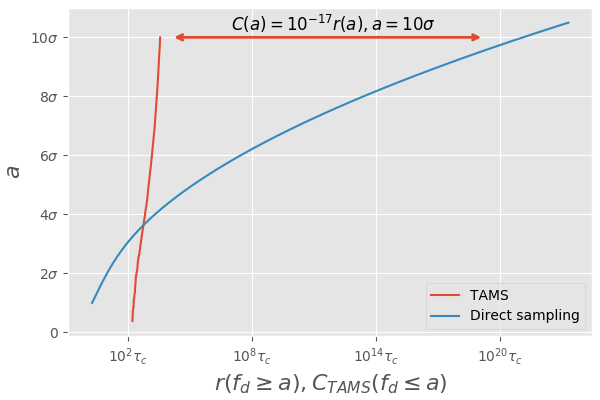
\includegraphics[width=.7\linewidth]{AMS_OU/AMS_OU.png}
  \caption{Efficiency of the \EL{\ac{ams} algorithm} with respect to direct sampling in the case of an Ornstein-Uhlenbeck process \citep{lestang_computing_2018}. The red line represents the evolution of the maximum obtained from re-sampled trajectories as a function of the computational cost $C_{AMS}$. The blue line is the analytical solution for the return time of amplitude $a$.}
  \label{fig:comparaison_temps_de_retour}
\end{figure}
Fluid dynamics is temporarily left aside and a one-dimensional \acl{ou} process is considered:
\begin{equation}
  \label{eq:ou}
  \dot{x} = -x + \eta (t),
\end{equation}
where $\eta$ is a Gaussian noise with $\langle \eta(t)\eta(t-t')\rangle = \delta(t-t')$.
This basic stochastic process will allow us to highlight differences with fluid dynamics.


The \ac{ams} is applied  to a set of $N=32$ trajectories $\{x_n(t)\}_{0\leq t \leq T_a}$ with $T_a=5\tau_c$.
Let us note that the correlation time is $\tau_c = 1$ for the process defined by Eq.~\eqref{eq:ou}.
Our objective is to sample fluctuations $x\geq a$ with $a$ being very large compared to the typical values of $x$.
The score function is simply $x(t)$ and a single trajectory is re-sampled at each iteration.

The computational cost of the algorithm after $J$ iterations is therefore related to the simulation of the $N$ initial trajectories and the re-sampling of $J$ trajectories.
Fig.~\ref{fig:comparaison_temps_de_retour} compares the computational cost of the \ac{ams} algorithm with that of a direct sampling.
In the latter, the typical computational cost is simply the return time $r(a)$.
One can see that the successive re-samplings of the \ac{ams} algorithm lead rapidly to trajectories exhibiting extreme fluctuations.
For large $a$, the computational cost is many orders of magnitude lower than that obtained by direct sampling.

Undoubtedly, the \acl{ou} process has oversimplified dynamics to showcase the efficiency of the \ac{ams} algorithm.
The state space is one-dimensional and the choice of the score function is straightforward: It is $x$ itself.
In addition, the noise term in Eq.~\eqref{eq:ou} has no correlation in time, which implies that newly generated trajectories quickly separate from their parents. Such favorable features \EL{do not} \textit{a priori} persist in the case of fluid dynamics.
  
%%% Local Variables:
%%% mode: latex
%%% TeX-master: "draft_p2_jfm"
%%% End:
